

\section{Normality Test}


In our analysis part, we use linear model to fit real data. There are several
assumptions on linear modeling, one of which is normality assumption on errors 
term. Normality of the errors can be checked by checking normality of the 
residuals. The usual way is plotting a Q-Q plot and check whether it forms a 
straight line. However in this paper, since there are around 200,000 voxels
it would be hard to plot all of them and check for normality. Thus we use 
Shapiro-Wilk test in the paper to test for normality. \par

In Shapiro-Wilk test, a small p-value indicates non-linearity. We write up a
function to compute p-value of each voxel and plot those p-values in three
brain perspectives. There are three linear models used in the paper, the below
6 plots are p-value plots, first three of them are p-values for three different
linear models using raw data. The other three plots are p-values for three 
different linear models using smoothed data. \par



\begin{figure}[h!]
\begin{subfigure}{.5\textwidth}
  \centering
  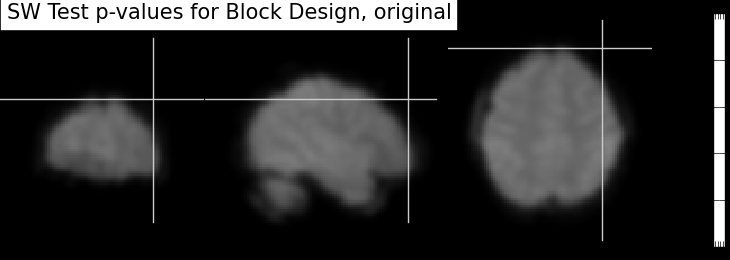
\includegraphics[width=.8\linewidth]{block_normality_test}
  \caption{Block Design, Original Data}
  \label{fig:block_origin}
\end{subfigure}%
\begin{subfigure}{.5\textwidth}
  \centering
  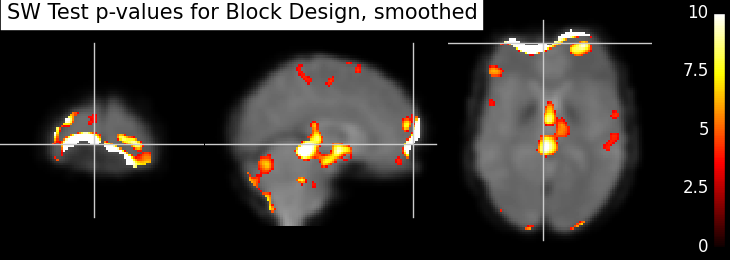
\includegraphics[width=.8\linewidth]{smoothed_block_normality_test}
  \caption{Block Design, Smoothed Data}
  \label{fig:block_smoothed}
\end{subfigure}
\begin{subfigure}{.5\textwidth}
  \centering
  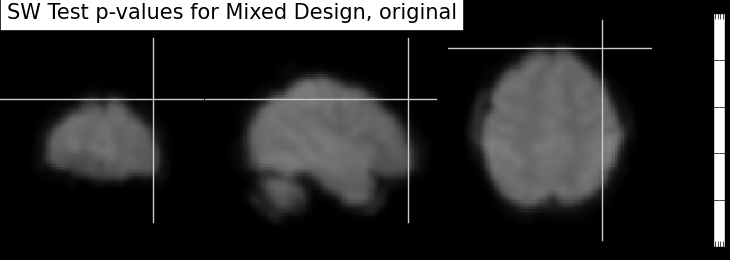
\includegraphics[width=.8\linewidth]{mixed_normality_test}
  \caption{Mixed Design, Original Data}
  \label{fig:mixed_origin}
\end{subfigure}%
\begin{subfigure}{.5\textwidth}
  \centering
  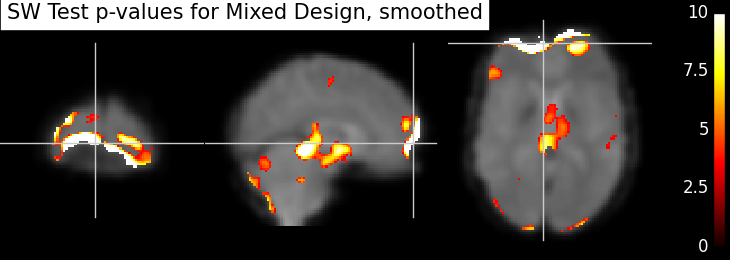
\includegraphics[width=.8\linewidth]{smoothed_mixed_normality_test}
  \caption{Mixed Design, Smoothed Data}
  \label{fig:mixed_smoothed}
\end{subfigure}
\begin{subfigure}{.5\textwidth}
  \centering
  
\includegraphics[width=.8\linewidth]{mixed_dct_normality_test}
  \caption{Mixed Design with DCT, Original Data}
  \label{fig:dct_origin}
\end{subfigure}%
\begin{subfigure}{.5\textwidth}
  \centering
  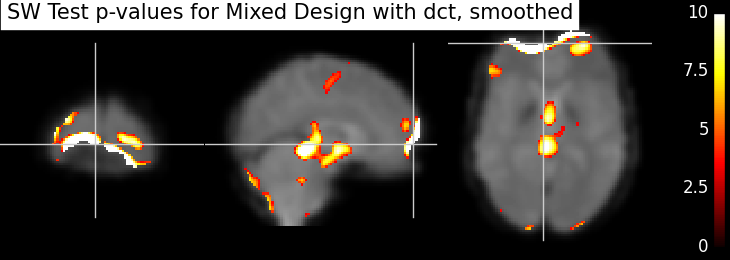
\includegraphics[width=.8\linewidth]{smoothed_mixed_dct_normality_test}
  \caption{Mixed Design with DCT, Smoothed Data}
  \label{fig:dct_origin}
\end{subfigure}
\caption{SW Test for Three Linear Models\label{fig:swtest}}
\end{figure}




The bright areas in the above plots means errors in that area don't follow
normal distribution. We can see that data before smoothed seems to follow
normal distribution well, while data after smoothed show some non-normality.
This makes sense, since there should be significant points for anatomy.





